% Information Flow Analysis of the Anoma EVM Protocol Adapter and ERC20 Forwarder Contracts
% Anoma Foundation — Security Research, April 2026

\documentclass[11pt,a4paper]{article}

%% ============================================================
%% Packages
%% ============================================================
%% Build: compile with XeLaTeX (uses fontspec + JetBrains Mono for code).
%%   xelatex report.tex   # run twice for cross-refs

\usepackage[margin=2.4cm]{geometry}
\usepackage{fontspec}
% Use default Latin Modern for main/sans (loaded automatically with fontspec)
% and JetBrains Mono for monospaced text. JetBrains Mono NL is the
% no-ligatures variant -- we use it for listings so source code renders
% character-for-character (no "->" glyph-merging).
\setmonofont{JetBrains Mono NL}[Scale=0.88]
\usepackage{microtype}
\usepackage{amsmath,amssymb}
\usepackage{booktabs}
\usepackage{array}
\usepackage{xcolor}
\usepackage{listings}
\usepackage{tikz}
\usetikzlibrary{arrows.meta,positioning,fit,backgrounds,calc,decorations.pathreplacing}
\usepackage[hidelinks,
  pdftitle={Information Flow Analysis of the Anoma EVM Protocol Adapter and ERC20 Forwarder},
  pdfauthor={Anoma Foundation --- Security Research},
  breaklinks=true]{hyperref}
\usepackage{cleveref}

% Allow long URLs to break at any character to prevent overfull hboxes.
\usepackage{xurl}
\Urlmuskip=0mu plus 1mu

%% ============================================================
%% Clickable GitHub source-code references
%%   \paref  / \parefR : Protocol Adapter files (single line / range)
%%   \fwdref / \fwdrefR: Forwarder files (single line / range) --
%%                       first arg is the subdirectory within contracts/src/
%%                       (use "" for the root, "bases/", "drafts/", ...)
%% Each macro resolves to a \texttt{file.sol:NN[-MM]} that links to the
%% corresponding line range on the main branch of the source repository.
%% ============================================================
\newcommand{\paRepoRoot}{https://github.com/anoma/pa-evm/blob/main/contracts/src}
\newcommand{\fwdRepoRoot}{https://github.com/anoma/anomapay-erc20-forwarder/blob/main/contracts/src}

\newcommand{\paref}[2]{\href{\paRepoRoot/#1\#L#2}{\nolinkurl{#1:#2}}}
\newcommand{\parefR}[3]{\href{\paRepoRoot/#1\#L#2-L#3}{\nolinkurl{#1:#2-#3}}}

\newcommand{\fwdref}[3]{\href{\fwdRepoRoot/#1#2\#L#3}{\nolinkurl{#2:#3}}}
\newcommand{\fwdrefR}[4]{\href{\fwdRepoRoot/#1#2\#L#3-L#4}{\nolinkurl{#2:#3-#4}}}

%% ============================================================
%% Colour palette
%% ============================================================
\definecolor{scifblue}{HTML}{1565C0}
\definecolor{soliditygray}{HTML}{374151}
\definecolor{commentgreen}{HTML}{388E3C}
\definecolor{keywordpurple}{HTML}{6A1B9A}
\definecolor{warnorange}{HTML}{E65100}
\definecolor{codebackground}{HTML}{F8F9FA}
\definecolor{critred}{HTML}{B71C1C}
\definecolor{highred}{HTML}{D32F2F}
\definecolor{medyellow}{HTML}{F57F17}

%% ============================================================
%% Listing styles
%% ============================================================

% SCIF language definition
\lstdefinelanguage{SCIF}{
  morekeywords={contract,interface,constructor,void,bytes,address,uint,bool,
    map,final,lock,atomic,rescue,endorse,emit,event,exception,throw,
    import,result,sender,this,super,assert,if,else,true,false,
    public,implements,returns},
  sensitive=true,
  morecomment=[l]{//},
  morecomment=[s]{/*}{*/},
  morestring=[b]",
}

% Solidity language definition
\lstdefinelanguage{Solidity}{
  morekeywords={pragma,solidity,contract,abstract,interface,library,
    function,returns,external,internal,public,private,override,virtual,
    immutable,constant,memory,calldata,storage,payable,view,pure,
    constructor,modifier,require,revert,emit,event,error,mapping,
    address,uint256,uint128,uint8,uint32,bytes32,bytes,bool,struct,enum,
    if,else,for,while,return,true,false,assembly,new,delete,unchecked},
  sensitive=true,
  morecomment=[l]{//},
  morecomment=[s]{/*}{*/},
  morestring=[b]",
}

\lstdefinestyle{scifstyle}{
  language=SCIF,
  backgroundcolor=\color{codebackground},
  basicstyle=\ttfamily\small,
  keywordstyle=\color{scifblue}\bfseries,
  commentstyle=\color{commentgreen}\itshape,
  stringstyle=\color{warnorange},
  numberstyle=\tiny\color{gray},
  numbers=left,
  numbersep=6pt,
  frame=single,
  framerule=0.4pt,
  rulecolor=\color{scifblue!40},
  breaklines=true,
  showstringspaces=false,
  tabsize=2,
  captionpos=b,
  xleftmargin=1.5em,
}

% Compact two-column listing styles (smaller font, no numbers, tight frame).
\lstdefinestyle{scifstyleCompact}{
  language=SCIF,
  backgroundcolor=\color{codebackground},
  basicstyle=\ttfamily\scriptsize,
  keywordstyle=\color{scifblue}\bfseries,
  commentstyle=\color{commentgreen}\itshape,
  stringstyle=\color{warnorange},
  frame=single,
  framerule=0.3pt,
  rulecolor=\color{scifblue!40},
  breaklines=true,
  showstringspaces=false,
  tabsize=2,
  numbers=none,
  xleftmargin=0.2em,
  xrightmargin=0.2em,
  aboveskip=2pt,
  belowskip=2pt,
}

\lstdefinestyle{soliditystyleCompact}{
  language=Solidity,
  backgroundcolor=\color{codebackground},
  basicstyle=\ttfamily\scriptsize,
  keywordstyle=\color{soliditygray}\bfseries,
  commentstyle=\color{commentgreen}\itshape,
  stringstyle=\color{warnorange},
  frame=single,
  framerule=0.3pt,
  rulecolor=\color{soliditygray!40},
  breaklines=true,
  showstringspaces=false,
  tabsize=2,
  numbers=none,
  xleftmargin=0.2em,
  xrightmargin=0.2em,
  aboveskip=2pt,
  belowskip=2pt,
}

\lstdefinestyle{soliditystyle}{
  language=Solidity,
  backgroundcolor=\color{codebackground},
  basicstyle=\ttfamily\small,
  keywordstyle=\color{soliditygray}\bfseries,
  commentstyle=\color{commentgreen}\itshape,
  stringstyle=\color{warnorange},
  numberstyle=\tiny\color{gray},
  numbers=left,
  numbersep=6pt,
  frame=single,
  framerule=0.4pt,
  rulecolor=\color{soliditygray!40},
  breaklines=true,
  showstringspaces=false,
  tabsize=4,
  captionpos=b,
  xleftmargin=1.5em,
}

%% ============================================================
%% Severity macros
%% ============================================================
\newcommand{\sevCrit}[1]{\textcolor{critred}{\textbf{[CRITICAL] #1}}}
\newcommand{\sevHigh}[1]{\textcolor{highred}{\textbf{[HIGH] #1}}}
\newcommand{\sevMed}[1]{\textcolor{medyellow}{\textbf{[MEDIUM] #1}}}

%% ============================================================
%% Title
%% ============================================================

\title{%
  \textbf{Information Flow Analysis of the\\
  Anoma EVM Protocol Adapter and ERC20 Forwarder}\\[0.6em]
  {\large\normalfont\itshape Research preview --- an exploratory SCIF study}%
  \thanks{All SCIF models and supplementary material at
    \texttt{information-flow-smart-contracts/}.}
}
\author{Anoma Foundation --- Security Research}
\date{April 2026}

%% ============================================================
\begin{document}
%% ============================================================

\maketitle

% Make the line breaker slightly more lenient (prevents protruding URLs /
% long typewriter words from causing overfull hboxes).
\sloppy
\emergencystretch=2em

%% ============================================================
\begin{abstract}
%% ============================================================

We present an information flow control (IFC) analysis of two interconnected
Anoma smart contracts: the EVM Protocol Adapter (\textsf{PA}), which verifies
RISC Zero zero-knowledge proofs and dispatches calls to registered forwarder
contracts, and the \textsf{ERC20Forwarder}, which wraps and unwraps ERC20 tokens
via Uniswap's Permit2 and manages a versioned emergency migration chain.
The analysis uses SCIF (Smart Contract Information Flow), a language that
compiles to Solidity and enforces integrity properties via the Decentralized
Label Model, preventing confused deputy attacks (CDAs), reentrancy violations,
and improper exception handling at the type level.

Six SCIF models were written covering the two contracts and their interactions.
The models surface \textbf{16 explicit endorsement sites} whose soundness
depends entirely on ZK circuit coverage --- a finding that is invisible to
conventional static analysis but becomes an enumerable audit checklist under
SCIF. Three findings of high or critical severity were identified: an emergency
committee architecture with no on-chain time-lock or multi-party gate that
permits single-actor fund drain (CRIT-1); the full CDA exposure introduced by
PA's user-controlled forwarder dispatch (HIGH-2); and a constructor-level
copy-paste error in \textsf{ERC20ForwarderV3} at line 77 that permanently
prevents migration of all V2 resources (HIGH). Three medium-severity and four
model gap findings complete the report. We discuss what SCIF catches that
conventional auditing tools miss, what it cannot catch, and the pitfalls that
arise when applying IFC to ZK-backed smart contracts.

\end{abstract}

%% ============================================================
\section*{Executive Summary}
\addcontentsline{toc}{section}{Executive Summary}
%% ============================================================

\paragraph{What we did.}
We rewrote the security-critical core of two Anoma smart contracts ---
the EVM Protocol Adapter (PA) and the ERC20 Forwarder --- in
SCIF~\cite{scif2025}, a language that compiles to Solidity and forces
every trust decision to be written down explicitly. The original
Solidity is silent about where untrusted user data becomes trusted;
the SCIF models name every such point. Six models were produced,
covering the PA, the forwarder, the emergency migration chain (V1--V3),
and the cross-contract call between PA and forwarder.

\paragraph{What we found.}
\begin{enumerate}
  \item \textbf{16 trust assumptions that depend on the ZK circuit}
    (HIGH-1). The PA endorses 6 user-supplied fields after proof
    verification; the forwarder endorses 10 more after checking
    \texttt{msg.sender == PA}. Each endorsement is only valid if the
    RISC Zero circuit constrains the corresponding field. No existing
    audit tool produces this list --- SCIF does.

  \item \textbf{Emergency committee can drain funds in two transactions}
    (CRIT-1). A single committee key can appoint an emergency caller
    who immediately drains all token balances. The contract enforces no
    time-lock or multi-party gate. Today this is mitigated off-chain by
    a multisig, but the contract itself provides no such guarantee.

  \item \textbf{Classic confused-deputy attack surface} (HIGH-2). The PA
    calls a forwarder address decoded from user calldata. If the ZK
    circuit does not constrain this address, an attacker can redirect PA
    calls to a malicious contract. An on-chain allowlist would eliminate
    this risk independent of the circuit.

  \item \textbf{V3 constructor bug} (HIGH). Line 77 of
    \texttt{ERC20ForwarderV3.sol} reads the commitment tree root from the
    wrong Protocol Adapter (V1 instead of V2). This permanently blocks
    migration of all V2 resources. Requires redeployment to fix.
\end{enumerate}

\paragraph{What to do next (priority order).}
\begin{enumerate}
  \item \textbf{Audit the ZK circuit against the 16-field checklist.}
    For each endorsed field, confirm it appears as a constrained output
    in the RISC Zero guest journal. Any missing field means an attacker
    controls that value despite the on-chain endorsement.

  \item \textbf{Add an on-chain forwarder allowlist} in the PA,
    independent of the ZK circuit.

  \item \textbf{Redeploy V3} with the corrected root read
    (\texttt{\_PROTOCOL\_ADAPTER\_V2} instead of \texttt{V1}).

  \item \textbf{Consider adding a time-lock} between
    \texttt{setEmergencyCaller} and the first
    \texttt{forwardEmergencyCall}.
\end{enumerate}

\paragraph{Scope and limitations.}
This is a \emph{research preview}, not a full audit. SCIF cannot analyze
the ZK circuit, economic attacks (MEV, sandwiching), gas griefing, or the
\texttt{abi.decode} step. The analysis complements --- not replaces --- the
existing Nethermind and Informal Systems audits. See
\cref{sec:gaps,sec:discussion} for details.

\bigskip
\tableofcontents
\bigskip

%% ============================================================
\section{Introduction}
%% ============================================================

Smart contract security audits typically proceed through a combination of
automated static analysis (Slither, Mythril, Halmos), formal verification of
isolated invariants, and manual review. Each of these approaches shares a
fundamental limitation: trust is \emph{implicit}. A Solidity variable carrying
user-supplied data is syntactically identical to a variable holding
protocol-level state; trust escalation occurs silently whenever untrusted data
is used in a privileged context.

Information flow control makes trust \emph{explicit}. Every value carries a
label that tracks where it came from and who may influence it. Every promotion
of an untrusted value to a trusted context requires an \texttt{endorse}
annotation --- a named, justified trust boundary that is visible, auditable, and
type-checked. The benefit for smart contract auditing is not merely that the
type-checker catches violations; it is that the complete set of trust boundaries
is enumerable, and that enumeration itself becomes an audit checklist.

This report documents the application of SCIF~\cite{scif2025} to two production
Anoma contracts. The primary contribution is not a list of novel attack
techniques --- most of the findings correspond to known vulnerability classes.
The contribution is demonstrating that SCIF's endorsement structure makes these
vulnerabilities \emph{structurally visible} rather than discoverable only
through expert pattern-matching, and that the ZK circuit dependency of those
endorsements --- entirely hidden in Solidity --- becomes an explicit, navigable
dependency graph.

\paragraph{Code under analysis.}
The Solidity contracts analysed in this report live in two public
repositories maintained by Anoma:
\begin{itemize}
  \item \textbf{Protocol Adapter}~\cite{paevmrepo} ---
    \href{https://github.com/anoma/pa-evm}{github.com/anoma/pa-evm}.
    Primary file:
    \href{https://github.com/anoma/pa-evm/blob/main/contracts/src/ProtocolAdapter.sol}{\texttt{ProtocolAdapter.sol}}.
  \item \textbf{ERC20 Forwarder}~\cite{forwarderrepo} ---
    \href{https://github.com/anoma/anomapay-erc20-forwarder}{github.com/anoma/anomapay-erc20-forwarder}.
    Primary files:
    \href{https://github.com/anoma/anomapay-erc20-forwarder/blob/main/contracts/src/ERC20Forwarder.sol}{\texttt{ERC20Forwarder.sol}},
    \href{https://github.com/anoma/anomapay-erc20-forwarder/blob/main/contracts/src/bases/ForwarderBase.sol}{\texttt{ForwarderBase.sol}},
    \href{https://github.com/anoma/anomapay-erc20-forwarder/blob/main/contracts/src/bases/EmergencyMigratableForwarderBase.sol}{\texttt{EmergencyMigratableForwarderBase.sol}},
    \href{https://github.com/anoma/anomapay-erc20-forwarder/blob/main/contracts/src/drafts/ERC20ForwarderV3.sol}{\texttt{ERC20ForwarderV3.sol}}.
\end{itemize}
The SCIF compiler is at
\href{https://github.com/apl-cornell/SCIF}{github.com/apl-cornell/SCIF}~\cite{scifrepo}.

\paragraph{Structure.} \Cref{sec:background} introduces the DLM, SCIF, and the
contracts under analysis. \Cref{sec:primer} is a SCIF primer for Solidity
developers: syntax cheat sheet, label semantics, a worked translation of
\texttt{ForwarderBase} from Solidity to SCIF, and instructions for running the
compiler. Readers already familiar with SCIF may skip it.
\Cref{sec:methodology} describes the modeling approach.
\Cref{sec:findings} presents all findings in severity order.
\Cref{sec:discussion} discusses what IFC catches, what it cannot, and the
pitfalls specific to this domain. \Cref{sec:glossary} defines key terms and
\Cref{sec:conclusion} gives recommendations.

%% ============================================================
\section{Background}
\label{sec:background}
%% ============================================================

\subsection{Information Flow Control for Smart Contracts}

IFC distinguishes two orthogonal security properties: \emph{confidentiality}
(data should not leak to unauthorized observers) and \emph{integrity} (only
authorized principals should be able to influence sensitive values). In smart
contracts the critical property is integrity: an attacker who can influence the
forwarder address dispatched by a protocol adapter, or the receiver address in
an unwrap operation, gains capabilities they were not authorized to hold.

SCIF enforces \emph{integrity} via the Decentralized Label
Model~\cite{myers1997sosp} (DLM). Each type carries a label, written $\{\pi\}$,
indicating which principal vouches for its integrity. Three labels appear
throughout this analysis:
\begin{itemize}
  \item $\{\texttt{this}\}$ --- the contract itself guarantees this value.
  \item $\{\texttt{sender}\}$ --- the current transaction sender supplied this
    value; it is untrusted.
  \item $\{\texttt{any}\}$ --- fully public, no integrity guarantee.
\end{itemize}
Trust escalation from $\{\texttt{sender}\}$ to $\{\texttt{this}\}$ requires an
explicit \texttt{endorse(x, sender -> this)} expression, which must be
justified by a runtime check (e.g., an access control guard or a cryptographic
verification step). This is the central discipline that SCIF imposes: every
trust promotion is named, located, and checkable.

SCIF prevents three vulnerability classes mechanically. SCIF builds on the
SeRIF calculus~\cite{serif2021}, which introduced lock-based compositional
reentrancy security; SCIF extends SeRIF with exception handling
(\texttt{atomic/rescue}) and adapts it to the smart-contract setting with
non-local control flow and transactions.
\begin{enumerate}
  \item \textbf{Confused Deputy Attacks (CDA).} If an untrusted address is used
    to dispatch a call with elevated authority, SCIF rejects the program unless
    the address has been endorsed to a trusted label first.
  \item \textbf{Reentrancy.} The $\texttt{lock}(\ell)$ construct holds a
    reentrancy lock at label $\ell$. After any external call inside a locked
    block, SCIF's \emph{program counter (PC) label} degrades unless the lock is
    maintained. State writes after an unprotected external call are rejected.
  \item \textbf{Improper exception handling.} The \texttt{atomic/rescue} blocks
    isolate failure: a revert inside \texttt{atomic} propagates to the
    \texttt{rescue} handler without leaving state inconsistent. SCIF ensures the
    PC label inside \texttt{rescue} reflects that a potentially attacker-induced
    failure has occurred.
\end{enumerate}

\subsection{The Anoma Protocol Adapter}

Following the Anoma specification~\cite{anomaspecs}, the Ethereum Virtual
Machine (EVM) protocol adapter is a smart contract written in Solidity that
can be deployed to EVM-compatible chains and roll-ups to connect them to the
Anoma protocol. It allows Anoma applications to run on existing EVM chains,
analogous to how drivers let an operating system run on different physical
hardware. The current prototype is \emph{settlement-only}: it processes
fully-evaluated transaction functions and does not implement the full executor
engine behaviour.

The Protocol Adapter (\textsf{PA}) maintains internal Resource Machine (RM)
state inside the contract, constituted by commitments, nullifiers, and blobs.
To interoperate with state in external contracts, the PA may, during
transaction execution, make read and write calls to \emph{forwarder
contracts}, which in turn translate those calls into reads and writes against
the external contracts they correspond to. A forwarder is only callable by the
protocol adapter, holds the address of the external contract it bridges, and
forwards arbitrary calls to it.

Concretely, the PA's \texttt{execute} function receives a \texttt{Transaction}
calldata value containing ZK proofs (generated and verified with RISC
Zero~\cite{anomaspecs}), nullifiers, commitments, logic references, and a
per-resource \emph{external payload} --- a variable-length array of
\texttt{(forwarderAddress, input, expectedOutput)} tuples. The PA verifies the
proofs, updates nullifiers and commitment tree roots, and calls
\texttt{IForwarder(untrustedForwarder).forwardCall(logicRef, input)} for each
payload entry.

The PA inherits \texttt{ReentrancyGuardTransient} (EIP-1153 transient
storage~\cite{eip1153}) and \texttt{Pausable} from OpenZeppelin. The
reentrancy guard is applied at the \texttt{execute} level. The PA holds no
token balances; it is a stateful verifier and dispatcher.

The trust model: the transaction submitter is untrusted; the RISC Zero
verifier router is an immutable trusted oracle; the forwarder contracts are
\emph{trusted by the PA only after the ZK proof certifies their address}.

\subsection{The ERC20 Forwarder}

The \textsf{ERC20Forwarder} holds ERC20 token balances on behalf of resource
owners. It exposes two operations:
\begin{itemize}
  \item \textbf{Wrap}: pull tokens from a user via Uniswap
    Permit2~\cite{permit2}, minting a resource commitment in the PA.
  \item \textbf{Unwrap}: push tokens to a receiver address, consuming a
    nullifier.
\end{itemize}
Access is gated by \texttt{msg.sender == \_PROTOCOL\_ADAPTER}, enforced in
\texttt{ForwarderBase.forwardCall}. The forwarder also inherits
\texttt{EmergencyMigratableForwarderBase}, which provides a two-step emergency
exit governed by an \texttt{\_EMERGENCY\_COMMITTEE} address.

\begin{figure}[h]
\centering
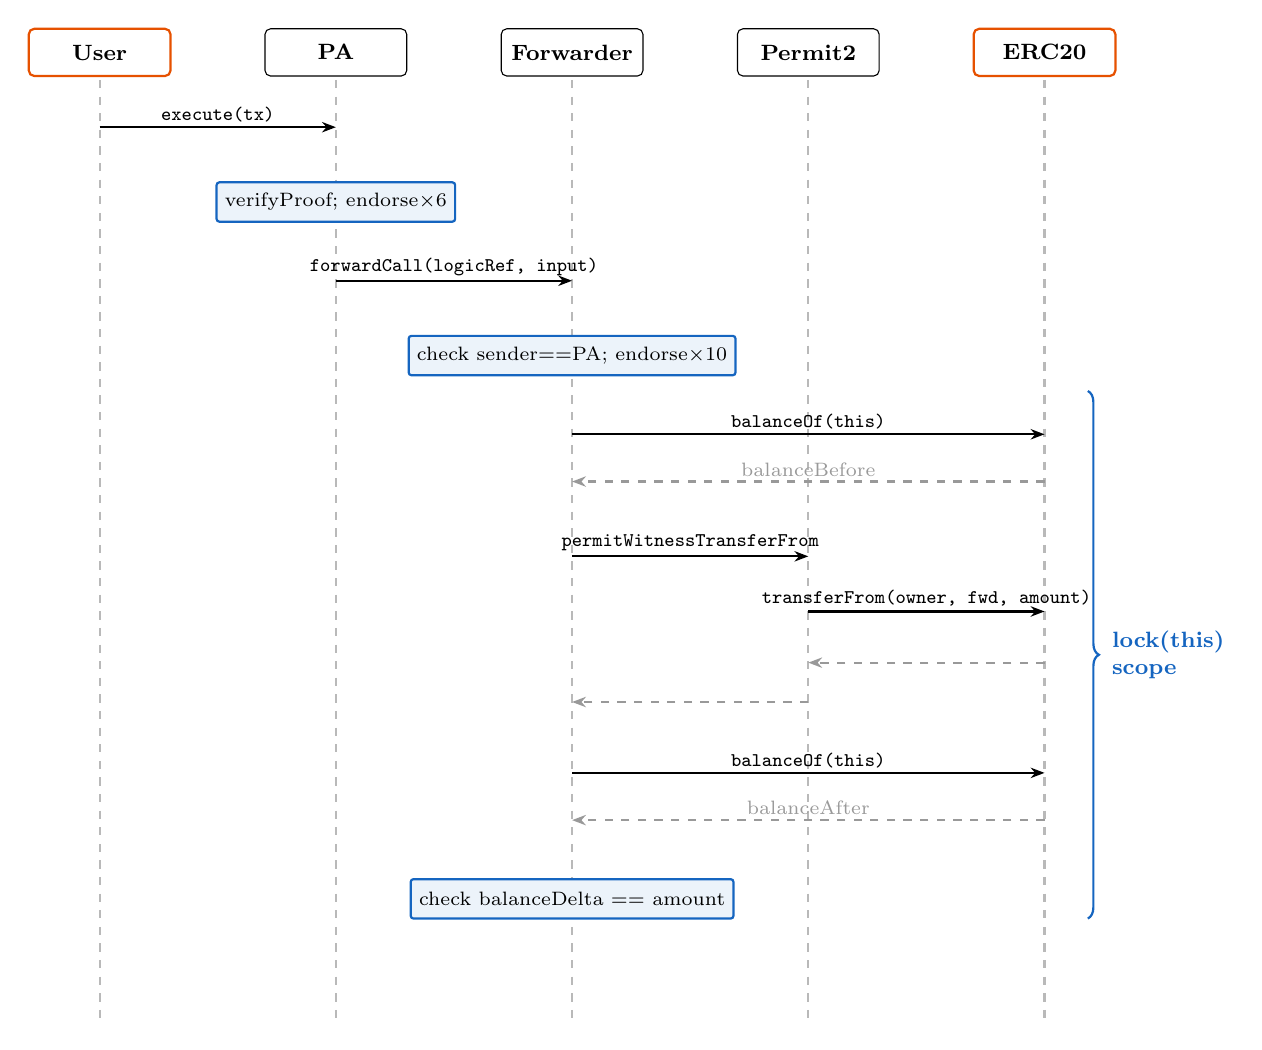
\begin{tikzpicture}[
  x=1cm,y=1cm,
  font=\footnotesize,
  lifeline/.style={draw=gray!55,dashed,thick},
  actor/.style={rectangle,draw,rounded corners=2pt,fill=white,
    minimum width=1.8cm,minimum height=0.6cm,align=center,font=\bfseries\footnotesize},
  untrustedactor/.style={actor,draw=warnorange,thick},
  action/.style={rectangle,draw=scifblue,thick,fill=scifblue!8,rounded corners=1pt,
    minimum height=0.5cm,inner sep=3pt,font=\scriptsize,align=center},
  msg/.style={-{Stealth[length=5pt]},thick},
  ret/.style={-{Stealth[length=5pt]},dashed,thick,gray!80},
  note/.style={font=\scriptsize,midway,above,inner sep=1.5pt},
]
%% 5 actors, 3cm spacing (total span 12cm, fits 16cm textwidth easily)
\node[untrustedactor] (u)  at (0, 0) {User};
\node[actor]          (p)  at (3, 0) {PA};
\node[actor]          (f)  at (6, 0) {Forwarder};
\node[actor]          (pm) at (9, 0) {Permit2};
\node[untrustedactor] (t)  at (12,0) {ERC20};

\foreach \x in {0,3,6,9,12} {
  \draw[lifeline] (\x,-0.35) -- (\x,-12.3);
}

\draw[msg] (0,-0.95) -- node[note]{\ttfamily execute(tx)} (3,-0.95);
\node[action] at (3,-1.9) {verifyProof; endorse$\times$6};
\draw[msg] (3,-2.9) -- node[note]{\ttfamily forwardCall(logicRef, input)} (6,-2.9);
\node[action] at (6,-3.85) {check sender==PA; endorse$\times$10};
\draw[msg] (6,-4.85) -- node[note]{\ttfamily balanceOf(this)} (12,-4.85);
\draw[ret] (12,-5.45) -- node[note]{balanceBefore} (6,-5.45);
\draw[msg] (6,-6.4) -- node[note]{\ttfamily permitWitnessTransferFrom} (9,-6.4);
\draw[msg] (9,-7.1) -- node[note]{\ttfamily transferFrom(owner, fwd, amount)} (12,-7.1);
\draw[ret] (12,-7.75) -- (9,-7.75);
\draw[ret] (9,-8.25) -- (6,-8.25);
\draw[msg] (6,-9.15) -- node[note]{\ttfamily balanceOf(this)} (12,-9.15);
\draw[ret] (12,-9.75) -- node[note]{balanceAfter} (6,-9.75);
\node[action] at (6,-10.75) {check balanceDelta == amount};

%% Lock(this) bracket on the right (inside textwidth)
\draw[decorate,decoration={brace,amplitude=4pt},scifblue,thick]
  (12.55,-4.3) -- node[midway,right,xshift=5pt,font=\footnotesize\bfseries,text=scifblue,align=left]
  {lock(this)\\scope} (12.55,-11.0);
\end{tikzpicture}
\caption{Wrap sequence with trust-label annotations. The balance invariant
(\texttt{balanceBefore} / \texttt{balanceAfter}) requires both reads and the
external calls to lie inside the same \texttt{lock(this)} scope; see
\cref{sec:med-balance}. The ERC20 actor (dashed orange) is user-controllable
--- a malicious token can execute arbitrary code during
\texttt{transferFrom} (GAP-2).}
\label{fig:wrap-msc}
\end{figure}

\paragraph{Migration chain.} The system supports contract upgrades through an
explicit versioned migration:
\[
  \text{V1 Forwarder} \;\xrightarrow{\text{migrate}}\;
  \text{V2 Forwarder} \;\xrightarrow{\text{migrate}}\;
  \text{V3 Forwarder}
\]
Each successor captures the predecessor's final commitment tree root at
construction time, uses this to validate migrating resources, and pulls token
balances forward via \texttt{forwardEmergencyCall}.

%% ============================================================
\section{A SCIF Primer for Solidity Developers}
\label{sec:primer}
%% ============================================================

Readers comfortable with SCIF may skip to \cref{sec:methodology}.
For everyone else, this section gives you enough to read every code listing
in the report. There are only three ideas you need.

\subsection{Three Labels}
\label{sec:primer-labels}

Every value in SCIF carries one of three labels that say \emph{who vouches
for it}:

\begin{description}
  \item[\texttt{\{this\}}] --- the \textbf{contract itself} guarantees this
    value (e.g., an immutable field set at deploy time).
  \item[\texttt{\{sender\}}] --- the \textbf{caller} supplied this value.
    It is untrusted until the contract explicitly accepts it.
  \item[\texttt{\{any\}}] --- \textbf{nobody} vouches for it. Fully public,
    no integrity guarantee.
\end{description}

In plain Solidity all three look the same: a \texttt{uint256} is a
\texttt{uint256} regardless of whether it came from calldata or from a
trusted storage slot. SCIF makes the difference visible.

\subsection{One Operation: \texttt{endorse}}
\label{sec:primer-endorse}

The only way to promote a value from \texttt{\{sender\}} to \texttt{\{this\}}
is to write an explicit \texttt{endorse}:

\begin{lstlisting}[style=scifstyle,numbers=none]
  uint{this} trustedAmount = endorse(amount, sender -> this);
\end{lstlisting}

This line says: ``I, the contract developer, accept responsibility for
treating \texttt{amount} as trusted from this point on.'' The SCIF compiler
checks that an \texttt{endorse} exists wherever it is needed. It does
\emph{not} check that the justification is correct --- that remains the
developer's job. The benefit is that every trust promotion becomes a named,
located line item that a reviewer can audit.

\subsection{One Rule: External Calls Drop Trust}
\label{sec:primer-pc}

After any external call (to a contract SCIF cannot analyze), SCIF assumes
the worst: the callee might have re-entered and changed state. So SCIF
\textbf{drops the trust level to \texttt{\{any\}}} after the call. Any
subsequent state write that requires \texttt{\{this\}} integrity is rejected.

To keep trust across an external call, wrap it in \texttt{lock(this)}.
This is SCIF's equivalent of Solidity's \texttt{nonReentrant} modifier,
but scoped to exactly the block that needs it:

\begin{lstlisting}[style=scifstyle,numbers=none]
  lock(this) {
      uint{this} before = tok.balanceOf(address(this));
      _wrap(token, amount, ...);       // external call
      uint{this} after = tok.balanceOf(address(this));
      // still trusted here because lock prevents re-entrance
  }
\end{lstlisting}

Without the lock, the second \texttt{balanceOf} read would be \texttt{\{any\}}
and the comparison with \texttt{amount} (which is \texttt{\{this\}}) would
fail at compile time. This is how SCIF catches reentrancy statically, and
why every external call in the models sits inside a \texttt{lock} block.

\subsection{Syntax Cheat Sheet}
\label{sec:primer-syntax}

\Cref{tab:scif-syntax} maps every SCIF construct used in this report to its
Solidity equivalent.

\begin{table}[h]
\centering
\caption{SCIF constructs used in this report.}
\label{tab:scif-syntax}
\small
\begin{tabular}{@{}p{4.8cm}p{4.3cm}p{5.2cm}@{}}
\toprule
\textbf{SCIF} & \textbf{Solidity} & \textbf{What it means} \\
\midrule
\texttt{address\{this\}} & \texttt{address} & Contract-trusted value. \\
\texttt{uint\{sender\}} & \texttt{uint256} (calldata) & Caller-supplied, untrusted. \\
\texttt{endorse(x, sender -> this)} & (nothing --- implicit) & Mark \texttt{x} as trusted. \\
\addlinespace
\texttt{lock(this) \{ ... \}} & \texttt{nonReentrant} scope & Keep trust across external calls. \\
\texttt{atomic \{ ... \} rescue * \{ ... \}} & \texttt{try/catch} & Isolate failure; trust drops inside \texttt{rescue}. \\
\addlinespace
\texttt{@public} & \texttt{external} & Anyone can call; reentrancy-locked. \\
\texttt{throw X()} & \texttt{revert X()} & Revert with a named error. \\
\texttt{sender} & \texttt{msg.sender} & Caller address. \\
\texttt{result = ...} & \texttt{return ...} & Return value. \\
\bottomrule
\end{tabular}
\end{table}

\subsection{Worked Example: ForwarderBase}
\label{sec:primer-example}

Here is the access-control function from \texttt{ForwarderBase}, first in
Solidity, then in SCIF. The SCIF version is only a few lines longer, but
it makes every trust decision visible.

\paragraph{Solidity (trust hidden).}

\begin{lstlisting}[style=soliditystyle,caption={\texttt{ForwarderBase.forwardCall} --- where does trust change?}]
function forwardCall(bytes32 logicRef, bytes calldata input)
    external returns (bytes memory)
{
    if (msg.sender != PROTOCOL_ADAPTER) revert UnauthorizedCaller();
    if (logicRef != LOGIC_REF) revert UnauthorizedLogicRef();
    return _forwardCall(input);  // input is treated as trusted here --- why?
}
\end{lstlisting}

A Solidity reader cannot tell \emph{from the code alone} where \texttt{input}
goes from untrusted to trusted. The answer is ``after the
\texttt{msg.sender} check,'' but that is an inference, not a visible mark.

\paragraph{SCIF (trust visible).}

\begin{lstlisting}[style=scifstyle,caption={Same function in SCIF --- every trust promotion is named.}]
@public
bytes{this} forwardCall(uint logicRef, bytes input)
    throws (UnauthorizedCaller, UnauthorizedLogicRef) {

    if (sender != _PROTOCOL_ADAPTER) { throw UnauthorizedCaller(); }

    // These two lines ARE the trust boundary:
    uint{this}  endorsedLogicRef = endorse(logicRef, sender -> this);
    bytes{this} endorsedInput    = endorse(input,    sender -> this);

    if (_LOGIC_REF != endorsedLogicRef) { throw UnauthorizedLogicRef(); }
    result = _forwardCall(endorsedInput);
}
\end{lstlisting}

The two \texttt{endorse} lines are the only place where untrusted data
becomes trusted. Remove either one and the program will not compile.
Across the whole codebase, listing every \texttt{endorse} gives you a
complete checklist of every trust assumption the contracts rely on ---
the central output of this report.

\subsection{The Same Idea, Applied to the Protocol Adapter}
\label{sec:primer-pa}

\texttt{ForwarderBase} only has two \texttt{endorse} sites. The PA has six,
because its trust boundary is a ZK proof instead of a simple caller check.
\Cref{fig:pa-sidebyside} puts the Solidity and SCIF versions of the PA's
core function side-by-side. The full source is in
\href{https://github.com/anoma/pa-evm/blob/main/contracts/src/ProtocolAdapter.sol}{\texttt{ProtocolAdapter.sol}}~\cite{paevmrepo};
the pipeline view is in \cref{fig:label-pipeline}.

\begin{figure}[h]
\noindent
\begin{minipage}[t]{0.48\textwidth}
\centering{\footnotesize\textbf{Solidity --- trust \emph{implicit}}}\\[2pt]
\begin{lstlisting}[style=soliditystyleCompact]
function execute(Transaction calldata tx)
    external nonReentrant whenNotPaused {

  _verifyProof(tx.proof);

  // No annotation: calldata fields are
  // used as if trusted from here on.
  _addNullifier(tx.nullifier);
  _addCommitment(tx.commitment);

  (address fwd,
   bytes memory input,
   bytes memory expOut) =
    abi.decode(tx.callBlob,
               (address, bytes, bytes));

  bytes memory out =
    IForwarder(fwd)
      .forwardCall(tx.logicRef, input);

  if (keccak256(out) != keccak256(expOut))
    revert OutputMismatch();
}
\end{lstlisting}
\end{minipage}%
\hfill
\begin{minipage}[t]{0.50\textwidth}
\centering{\footnotesize\textbf{SCIF --- trust \emph{explicit}}}\\[2pt]
\begin{lstlisting}[style=scifstyleCompact]
@public
void execute(uint nullifier, uint commitment,
    uint logicRef, address forwarderAddr,
    bytes forwarderInput, bytes expectedOutput,
    bytes proof) throws (...) {

  // 1. ZK verifier is a declared oracle:
  bytes{this} eProof =
    endorse(proof, sender -> this);
  _verifyProof(eProof);

  // 2. Six post-oracle endorsements
  //    == the HIGH-1 checklist:
  uint{this}    eNull = endorse(nullifier,
                                sender -> this);
  uint{this}    eComm = endorse(commitment,
                                sender -> this);
  uint{this}    eLR   = endorse(logicRef,
                                sender -> this);
  address{this} eFwd  = endorse(forwarderAddr,
                                sender -> this);
  bytes{this}   eIn   = endorse(forwarderInput,
                                sender -> this);
  bytes{this}   eOut  = endorse(expectedOutput,
                                sender -> this);

  // 3. State + ext. call in ONE lock scope:
  lock(this) {
    if (_nullifiers[eNull])
      throw NullifierAlreadyExists();
    _nullifiers[eNull] = true;
    _commitmentCount = _commitmentCount + 1;
    _executeForwarderCall(
      eLR, eFwd, eIn, eOut);
  }
}
\end{lstlisting}
\end{minipage}
\caption{Side-by-side comparison of the PA's trust-critical core. Left: the
Solidity reader cannot tell which calldata fields are attacker-influenced or
where trust is granted. Right: each \texttt{endorse(x, sender -> this)} names
the field, localizes the trust promotion, and produces a line item in the
16-endorsement checklist described in HIGH-1. The \texttt{lock(this)} block
scopes the reentrancy discipline to exactly the state writes that require
it.}
\label{fig:pa-sidebyside}
\end{figure}

\paragraph{What this shows.}
On the left (Solidity), six calldata fields are used after
\texttt{\_verifyProof} with no visible mark that they just crossed a trust
boundary. On the right (SCIF), each \texttt{endorse} line names the field
and marks exactly where trust is granted. Listing all six gives you a
one-to-one checklist: each field must be a constrained output of the ZK
circuit. That checklist is the basis of finding HIGH-1 (\cref{sec:high1})
and the pipeline in \cref{fig:label-pipeline}.

The \texttt{lock(this)} block at the bottom scopes the reentrancy
protection to exactly the state writes and external call that need it ---
if the scope were too narrow, SCIF would reject the program.

\subsection{Running the SCIF Compiler}
\label{sec:primer-running}

The artefact repository provides a \texttt{justfile} and a GitHub Actions
workflow for reproducing the analysis.

\paragraph{Prerequisites.}
\begin{itemize}
  \item Java 21 (Temurin distribution recommended).
  \item A checkout of the SCIF compiler from
    \texttt{github.com/apl-cornell/SCIF}, placed at \texttt{\$SCIF\_DIR}
    (default: \texttt{../forks/SCIF} relative to the artefact root).
  \item The \texttt{just} command runner (\texttt{brew install just} on
    macOS; package manager on Linux).
\end{itemize}

\paragraph{Common commands.}
\begin{itemize}
  \item \texttt{just check} --- verify that Java and the SCIF compiler are
    reachable.
  \item \texttt{just typecheck-all} --- run the SCIF type-checker over every
    \texttt{.scif} file in the repository.
  \item \texttt{just compile-all} --- compile every \texttt{.scif} file to
    Solidity; output is written to \texttt{tmp/}.
  \item \texttt{just typecheck forwarder/ForwarderBase.scif} --- type-check a
    single model.
\end{itemize}

\paragraph{Continuous integration.}
The workflow at \texttt{.github/workflows/scif-check.yml} runs
\texttt{typecheck-all} and \texttt{compile-all} on every push and pull
request, uploading the generated Solidity as a build artefact. Failures in
either step fail the build, so the SCIF models stay in sync with the
repository across contributions.

%% ============================================================
\section{Methodology}
\label{sec:methodology}
%% ============================================================

\subsection{SCIF Modeling Approach}

The models are not line-for-line rewrites. The goal is to extract the
\emph{trust-critical core}: the paths through which user-supplied data reaches
state-modifying operations or external calls with elevated authority. Solidity
features not relevant to IFC (event emission gas optimization, library
delegation, complex struct packing) are omitted. Solidity features that
\emph{cannot} be expressed in SCIF are documented as explicit limitations with
justifications for why the omission does not affect the IFC conclusions.

\paragraph{Key limitations worked around.}
\begin{itemize}
  \item \textbf{No \texttt{final} fields in constructors.} SCIF's
    \texttt{final} qualifier requires declaration-site initialization.
    All immutable addresses are modeled as \texttt{address\{this\}} with
    constructor-time \texttt{endorse} to achieve the same integrity label.
  \item \textbf{No \texttt{bytes32}.} All byte hashes (nullifiers, logic
    references, commitment roots) are modeled as \texttt{uint}. Labels are
    unaffected since SCIF's integrity tracking is type-independent.
  \item \textbf{No \texttt{abi.decode}.} The real contracts decode calldata
    inline. The SCIF models receive already-decoded parameters, abstracting the
    decode step. This is a model gap documented in \cref{sec:gap1}.
  \item \textbf{No struct types.} \texttt{WrapData} and \texttt{UnwrapData} are
    flattened into individual parameters. This changes the function signature
    but not the IFC conclusions.
  \item \textbf{External calls forbidden before \texttt{super()} in
    constructors.} Constructors that read external contract state (e.g.,
    \texttt{latestCommitmentTreeRoot()}) must initialize fields with placeholder
    \texttt{endorse(0, sender -> this)} values, call \texttt{super()}, then
    overwrite them. This is a structural constraint with no semantic impact.
\end{itemize}

\paragraph{Label assignment strategy.} Constructor arguments from the deployer
are endorsed \texttt{sender -> this} immediately; the deployer is trusted to
configure the system correctly. User transaction parameters are tagged
$\{\texttt{sender}\}$ and remain at that label until the ZK proof verification
oracle approves them, at which point they are endorsed to
$\{\texttt{this}\}$. Access-gated parameters (from the PA calling the
forwarder, from the committee calling emergency functions) are endorsed after
the runtime check that verifies the caller's identity.

\subsection{Models Created}

\Cref{tab:models} lists the six SCIF models produced, with endorsement counts
and dynamic call counts as compiled by the SCIF type-checker.

\begin{table}[h]
\centering
\caption{SCIF models: endorsement and dynamic call counts.}
\label{tab:models}
\small
\begin{tabular}{@{}lrrl@{}}
\toprule
\textbf{Model file} & \textbf{Endorsements} & \textbf{Dyn.\ calls} & \textbf{Notes} \\
\midrule
\texttt{ForwarderBase.scif}           & 4  & 4  & Base access-control pattern \\
\texttt{ProtocolAdapterCore.scif}     & 9  & 6  & ZK oracle; 6 post-proof endorsements \\
\texttt{PaAndForwarder.scif}          & 10 & 6  & Cross-contract CDA trace \\
\texttt{ERC20Forwarder.scif}          & 13 & 6  & 10 wrap/unwrap param endorsements \\
\texttt{EmergencyMigratableBase.scif} & 5  & 10 & Committee governance chain \\
\texttt{ERC20ForwarderV3.scif}        & 14 & 12 & V3 bug visible in endorsement \\
\midrule
\textbf{Total}                        & \textbf{55} & \textbf{44} & 16 post-oracle sites \\
\bottomrule
\end{tabular}
\end{table}

The 16 ``post-oracle'' endorsement sites are those that follow ZK proof
verification and therefore derive their soundness entirely from the RISC Zero
circuit. Six appear in \texttt{ProtocolAdapterCore.scif} and ten appear in
\texttt{ERC20Forwarder.scif}. These are the primary subject of \cref{sec:high1}.

%% ============================================================
\section{Findings}
\label{sec:findings}
%% ============================================================

\subsection{CRIT-1: Emergency Committee Is a Single-Actor Fund Drain}
\label{sec:crit1}

\paragraph{Attack scenario.}
The \texttt{\_EMERGENCY\_COMMITTEE} address (immutable, set at deploy time)
calls \texttt{setEmergencyCaller(attackerAddr)} once the PA is stopped.
The attacker's address immediately becomes \texttt{\_emergencyCaller}. One
additional transaction calling \texttt{forwardEmergencyCall(input)} with a
\texttt{Unwrap} calltype drains the forwarder's entire token balance. The
complete attack is two transactions with no on-chain delay.

\paragraph{Affected code.}
\begin{itemize}
  \item Solidity: \fwdrefR{bases/}{EmergencyMigratableForwarderBase.sol}{55}{68}
    (\texttt{setEmergencyCaller}) and
    \fwdrefR{bases/}{EmergencyMigratableForwarderBase.sol}{42}{52}
    (\texttt{forwardEmergencyCall}).
  \item SCIF: \texttt{EmergencyMigratableBase.scif:129--164} and
    \texttt{188--224}.
\end{itemize}

\paragraph{How SCIF surfaces this.}
The label chain is single-step and unambiguous:

\begin{lstlisting}[style=scifstyle,caption={Emergency governance label chain in \texttt{EmergencyMigratableBase.scif}.}]
// setEmergencyCaller: committee check then one-step endorsement
if (sender != _EMERGENCY_COMMITTEE) {
    throw UnauthorizedCaller();
}
// Write-once guard: runtime only, not a label property
if (_emergencyCaller != address(0)) {
    throw EmergencyCallerAlreadySet();
}
// SINGLE TRUST ESCALATION: committee -> contract integrity
address{this} endorsedCaller = endorse(newEmergencyCaller, sender -> this);
_emergencyCaller = endorsedCaller;
\end{lstlisting}

\begin{lstlisting}[style=scifstyle,caption={Fund drain path: emergency caller with unrestricted input.}]
// forwardEmergencyCall: caller check then unconditional drain
if (sender != _emergencyCaller) { throw UnauthorizedCaller(); }
bytes{this} endorsedInput = endorse(input, sender -> this);
lock(this) {
    atomic {
        result = _forwardEmergencyCallInternal(endorsedInput); // arbitrary token op
    } rescue * { ... }
}
\end{lstlisting}

The endorsement chain is:
\[
  \underbrace{\texttt{\_EMERGENCY\_COMMITTEE}}_{\{this\}}
  \xrightarrow{\texttt{setEmergencyCaller}}
  \underbrace{\texttt{\_emergencyCaller}}_{\{this\}}
  \xrightarrow{\texttt{forwardEmergencyCall}}
  \text{drain all tokens}
\]
There is no intermediate endorser, no time-lock, no second principal. In
Solidity this structure is present but implicit. In SCIF the single-step
escalation is inescapably visible in the endorsement annotation.

\begin{figure}[h]
\centering
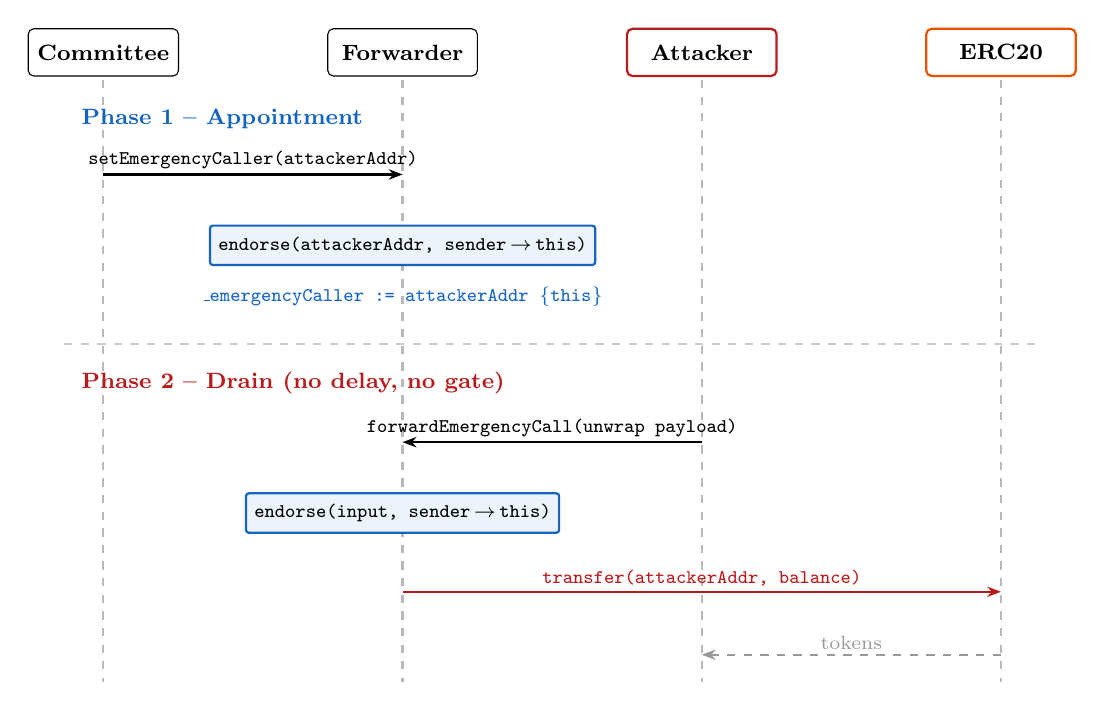
\begin{tikzpicture}[
  x=1cm,y=1cm,
  font=\footnotesize,
  lifeline/.style={draw=gray!55,dashed,thick},
  actor/.style={rectangle,draw,rounded corners=2pt,fill=white,
    minimum width=1.9cm,minimum height=0.6cm,align=center,font=\bfseries\footnotesize},
  badactor/.style={actor,draw=critred,thick},
  tokenactor/.style={actor,draw=warnorange,thick},
  action/.style={rectangle,draw=scifblue,thick,fill=scifblue!8,rounded corners=1pt,
    minimum height=0.5cm,inner sep=3pt,font=\scriptsize,align=center},
  msg/.style={-{Stealth[length=5pt]},thick},
  drain/.style={-{Stealth[length=5pt]},thick,critred},
  ret/.style={-{Stealth[length=5pt]},dashed,thick,gray!80},
  note/.style={font=\scriptsize,midway,above,inner sep=1.5pt},
  phasebar/.style={font=\footnotesize\bfseries,text=scifblue},
]
%% 4 actors, 3.8cm spacing -> total span 11.4cm
\node[actor]      (c) at (0,   0) {Committee};
\node[actor]      (f) at (3.8, 0) {Forwarder};
\node[badactor]   (a) at (7.6, 0) {Attacker};
\node[tokenactor] (e) at (11.4,0) {ERC20};

\foreach \x in {0,3.8,7.6,11.4} {
  \draw[lifeline] (\x,-0.35) -- (\x,-8.0);
}

\node[phasebar,anchor=west] at (-0.4,-0.85) {Phase 1 -- Appointment};
\draw[msg] (0,-1.55) -- node[note]{\ttfamily setEmergencyCaller(attackerAddr)} (3.8,-1.55);
\node[action] (fa1) at (3.8,-2.45) {\ttfamily endorse(attackerAddr, sender\,$\to$\,this)};
\node[font=\scriptsize\ttfamily,text=scifblue] at (3.8,-3.1) {\_emergencyCaller := attackerAddr \{this\}};

\draw[gray!40,dashed,thick] (-0.5,-3.7) -- (11.9,-3.7);

\node[phasebar,anchor=west,text=critred] at (-0.4,-4.2) {Phase 2 -- Drain (no delay, no gate)};
\draw[msg] (7.6,-4.95) -- node[note]{\ttfamily forwardEmergencyCall(unwrap payload)} (3.8,-4.95);
\node[action] (fa2) at (3.8,-5.85) {\ttfamily endorse(input, sender\,$\to$\,this)};
\draw[drain] (3.8,-6.85) -- node[note]{\ttfamily transfer(attackerAddr, balance)} (11.4,-6.85);
\draw[ret] (11.4,-7.65) -- node[note]{tokens} (7.6,-7.65);
\end{tikzpicture}
\caption{Emergency governance drain sequence. Between Phase~1 and Phase~2 the
contract enforces no on-chain delay or additional confirmation; a single
committee-key compromise enables a two-transaction fund drain. The SCIF
endorsement at \texttt{EmergencyMigratableBase.scif:163} is the only trust
promotion between the committee and \texttt{\_emergencyCaller}.}
\label{fig:emergency-msc}
\end{figure}

\paragraph{Severity assessment.} The committee is, by design, the root of
trust for the emergency path. Whether this is acceptable depends on the
deployment's governance model. At the time of writing the emergency caller
is operated as an off-chain multisig with a small number of signers (one to
two), so a single key compromise does not translate to a single-signer drain
in practice. The SCIF finding still applies because the contract itself
encodes no such constraint: the endorsement from \texttt{\{sender\}} to
\texttt{\{this\}} is unconditional once \texttt{sender == \_EMERGENCY\_COMMITTEE}
holds, and the number or composition of signers behind that address is a
purely off-chain property. A future reduction of the signer set, or a change
of custody, would not require any on-chain change.

\paragraph{Mitigation.} Add a time-lock between \texttt{setEmergencyCaller}
and the first permitted \texttt{forwardEmergencyCall} invocation (e.g., a
block-number-based delay stored at \texttt{setEmergencyCaller} time). A second
endorser in the SCIF model would represent a multi-sig threshold requirement.

\subsection{HIGH-1: ZK Circuit Gaps Make All 16 PA Endorsements Unsound by Default}
\label{sec:high1}

\paragraph{The oracle assumption.}
PA's \texttt{execute} endorses six fields to $\{\texttt{this}\}$ after
\texttt{\_verifyProof} returns without reverting.
\texttt{ERC20Forwarder.forwardCall} endorses ten fields after confirming
\texttt{sender == \_PROTOCOL\_ADAPTER}. The soundness of all 16 endorsements
depends on the RISC Zero circuit covering those fields as constrained public
inputs in its journal. SCIF cannot reach inside the circuit. This is modeled as
an oracle: if the verifier accepts, we endorse.

\begin{lstlisting}[style=scifstyle,caption={Six post-proof endorsements in \texttt{ProtocolAdapterCore.scif:89--94}.}]
// After _verifyProof returns: trust is granted to all fields
uint{this}    eNullifier  = endorse(nullifier,     sender -> this);
uint{this}    eCommitment = endorse(commitment,    sender -> this);
uint{this}    eLogicRef   = endorse(logicRef,      sender -> this);
address{this} eForwarder  = endorse(forwarderAddr, sender -> this);
bytes{this}   eInput      = endorse(forwarderInput,sender -> this);
bytes{this}   eExpected   = endorse(expectedOutput,sender -> this);
\end{lstlisting}

\begin{lstlisting}[style=scifstyle,caption={Ten post-access-check endorsements in \texttt{ERC20Forwarder.scif:147--156}.}]
// After sender == _PROTOCOL_ADAPTER check:
uint{this}    eCallType = endorse(callType,   sender -> this);
address{this} eToken    = endorse(token,      sender -> this);
uint{this}    eAmount   = endorse(amount,     sender -> this);
uint{this}    eNonce    = endorse(nonce,      sender -> this);
uint{this}    eDeadline = endorse(deadline,   sender -> this);
address{this} eOwner    = endorse(owner,      sender -> this);
uint{this}    eWitness  = endorse(witness,    sender -> this);
bytes{this}   eSig      = endorse(signature,  sender -> this);
address{this} eReceiver = endorse(receiver,   sender -> this);
// (eLogicRef endorsed separately)
\end{lstlisting}

\paragraph{Risk.} If the RISC Zero guest program does not constrain
\texttt{forwarderAddr} as a journal output, the attacker can supply any
address in the transaction calldata and receive a PA-authorized call to it ---
the CDA described in \cref{sec:high2}. If \texttt{receiver} in an unwrap
operation is unconstrained, the attacker directs token withdrawal to an
arbitrary address. Neither of these is detectable by inspecting the Solidity
contracts.

\begin{figure}[h]
\centering
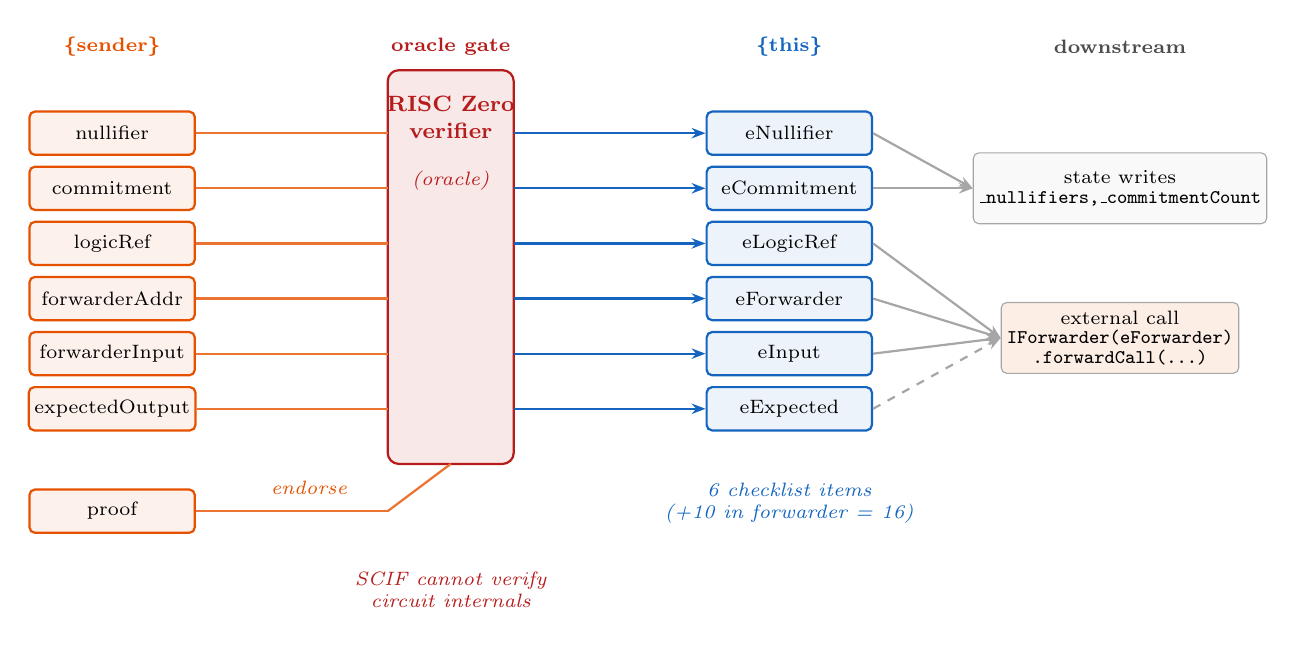
\begin{tikzpicture}[
  x=1cm,y=1cm,
  font=\footnotesize,
  box/.style={rectangle,draw,rounded corners=2pt,align=center,
    minimum height=0.55cm,minimum width=2.1cm,inner sep=2pt,font=\scriptsize},
  untrusted/.style={box,draw=warnorange,thick,fill=warnorange!8},
  trusted/.style={box,draw=scifblue,thick,fill=scifblue!8},
  downstream/.style={box,draw=gray!70,fill=gray!5,
    minimum width=2.7cm,minimum height=0.9cm},
  inarrow/.style={-{Stealth[length=5pt]},thick,warnorange!80},
  outarrow/.style={-{Stealth[length=5pt]},thick,scifblue},
  dsarrow/.style={-{Stealth[length=5pt]},thick,gray!70},
]
%% ---- Oracle drawn FIRST so arrows render on top of it and appear to
%%      pass through it as a gate. ----
\path[fill=critred!10,draw=critred,thick,rounded corners=4pt]
  (3.5,-0.7) rectangle (5.1, 4.3);
\node[font=\bfseries\footnotesize,text=critred,align=center]
  at (4.3, 3.7) {RISC Zero\\verifier};
\node[font=\scriptsize\itshape,text=critred] at (4.3, 2.9) {(oracle)};

%% ---- Column headers ----
\node[font=\bfseries\scriptsize,text=warnorange] at (0,   4.6) {\{sender\}};
\node[font=\bfseries\scriptsize,text=critred]    at (4.3, 4.6) {oracle gate};
\node[font=\bfseries\scriptsize,text=scifblue]   at (8.6, 4.6) {\{this\}};
\node[font=\bfseries\scriptsize,text=black!70]   at (12.8,4.6) {downstream};

%% ---- Left: 6 untrusted inputs (rows 0.70 apart) ----
\node[untrusted] (n1) at (0, 3.50) {nullifier};
\node[untrusted] (n2) at (0, 2.80) {commitment};
\node[untrusted] (n3) at (0, 2.10) {logicRef};
\node[untrusted] (n4) at (0, 1.40) {forwarderAddr};
\node[untrusted] (n5) at (0, 0.70) {forwarderInput};
\node[untrusted] (n6) at (0, 0.00) {expectedOutput};

%% ---- Right: 6 endorsed fields (same y-coordinates) ----
\node[trusted] (e1) at (8.6, 3.50) {eNullifier};
\node[trusted] (e2) at (8.6, 2.80) {eCommitment};
\node[trusted] (e3) at (8.6, 2.10) {eLogicRef};
\node[trusted] (e4) at (8.6, 1.40) {eForwarder};
\node[trusted] (e5) at (8.6, 0.70) {eInput};
\node[trusted] (e6) at (8.6, 0.00) {eExpected};

%% ---- Arrows: each endorsement is TWO segments ----
%%      1) {sender} field -> oracle's LEFT edge (orange, no head)
%%      2) oracle's RIGHT edge -> {this} field (blue, with head)
\foreach \s/\d/\y in {n1/e1/3.50,n2/e2/2.80,n3/e3/2.10,
                       n4/e4/1.40,n5/e5/0.70,n6/e6/0.00} {
  \draw[inarrow,-]   (\s.east) -- (3.5,\y);
  \draw[outarrow]    (5.1,\y)  -- (\d.west);
}

%% ---- Proof enters oracle separately from below ----
\node[untrusted] (np) at (0,-1.30) {proof};
\draw[inarrow,-] (np.east) -- (3.5,-1.30);
\draw[inarrow,-] (3.5,-1.30) -- (4.3,-0.7);  %% up into oracle bottom
\node[font=\scriptsize\itshape,text=warnorange] at (2.5,-1.0) {endorse};

%% ---- Downstream boxes ----
\node[downstream] (state) at (12.8, 2.8)
  {state writes\\[-1pt]\scriptsize\ttfamily \_nullifiers,\_commitmentCount};
\node[downstream,fill=warnorange!10] (fwd) at (12.8, 0.9)
  {external call\\[-1pt]\scriptsize\ttfamily IForwarder(eForwarder)\\[-1pt]\scriptsize\ttfamily .forwardCall(...)};

\draw[dsarrow] (e1.east) -- (state.west);
\draw[dsarrow] (e2.east) -- (state.west);
\draw[dsarrow] (e3.east) -- (fwd.west);
\draw[dsarrow] (e4.east) -- (fwd.west);
\draw[dsarrow] (e5.east) -- (fwd.west);
\draw[dsarrow,dashed] (e6.east) -- (fwd.west);

%% ---- Bottom annotations (non-overlapping) ----
\node[font=\scriptsize\itshape,text=critred,align=center] at (4.3,-2.3)
  {SCIF cannot verify\\circuit internals};
\node[font=\scriptsize\itshape,text=scifblue,align=center] at (8.6,-1.2)
  {6 checklist items\\(+10 in forwarder = 16)};
\end{tikzpicture}
\caption{Label pipeline through \texttt{ProtocolAdapterCore.execute}. Six
user-supplied fields (left, \{sender\}) and the proof enter the RISC Zero
verifier gate (centre) and emerge as six endorsed \{this\} values (right).
The orange segments are untrusted; the blue segments are trusted. Each
left/right pair is one mandatory \texttt{endorse} site, sound only if the
ZK circuit covers the corresponding journal output. The ten additional
endorsement sites in the ERC20 forwarder (total: 16) form the full checklist
described in HIGH-1.}
\label{fig:label-pipeline}
\end{figure}

\paragraph{Why SCIF adds value.} By producing an exact list of the 16
endorsement sites, SCIF generates a one-to-one checklist: each endorsed field
must correspond to a named, constrained public output in the RISC Zero guest's
journal. This is a verification task that is mechanically conceivable only
because SCIF enumerates the sites.

\paragraph{Mitigation.} Audit each of the 16 fields against the RISC Zero guest
journal. For each field, confirm it appears as a constrained output. Fields that
do not appear in the journal should be considered attacker-controlled regardless
of the on-chain endorsement.

\subsection{HIGH-2: Confused Deputy Attack via User-Controlled Forwarder Address}
\label{sec:high2}

\paragraph{The Dexible pattern.}
In February 2023, the Dexible protocol lost \$2M because its aggregator
contract accepted a user-supplied swap router address and called it with
Dexible's own identity --- a classic CDA~\cite{dexible2023}. The Anoma PA
architecture instantiates the same pattern: the forwarder address is decoded
from user-supplied calldata (\parefR{ProtocolAdapter.sol}{321}{322}) and passed
to \texttt{IForwarder(untrustedForwarder).forwardCall(...)}, where
\texttt{msg.sender == PA}. A malicious contract at \texttt{untrustedForwarder}
passes the \texttt{\_checkCaller(\_PROTOCOL\_ADAPTER)} access check in any
registered forwarder, because the check is against \texttt{msg.sender} and
\texttt{msg.sender} is the PA.

\begin{lstlisting}[style=soliditystyle,caption={\protect\parefR{ProtocolAdapter.sol}{320}{326}: forwarder decoded from calldata, no allowlist.}]
function _executeForwarderCall(
    bytes32 carrierLogicRef, bytes calldata callBlob
) internal {
    (address untrustedForwarder, bytes memory input, bytes memory expectedOutput)
        = abi.decode(callBlob, (address, bytes, bytes));
    bytes memory actualOutput =
        IForwarder(untrustedForwarder).forwardCall({
            logicRef: carrierLogicRef, input: input
        });
    // ...
}
\end{lstlisting}

\paragraph{How SCIF surfaces this.}
The combined model \texttt{PaAndForwarder.scif} makes the full call chain
appear in a single file. The comment at line 109 of \texttt{ProtocolAdapterCore.scif}
reads: ``CDA risk: if the ZK circuit allows the user to specify a malicious
forwarder address, the PA would call it with full PA authority.'' SCIF requires
the developer to write this trust boundary as an \texttt{endorse} call; the
comment is a mandatory documentation checkpoint.

\paragraph{Current mitigation status.}
The ZK circuit is expected to constrain the forwarder address to a fixed
allowlist. SCIF cannot verify this; the endorsement is sound only if the circuit
does constrain the address. This creates a dependency between the on-chain
security of the PA and the correctness of off-chain ZK circuit design --- a
dependency that is invisible in Solidity but explicit in the SCIF model.

\paragraph{Mitigation.} Maintain an on-chain registry of approved forwarder
addresses in the PA with a runtime \texttt{require} check before
\texttt{forwardCall}, independent of the ZK circuit. This eliminates the oracle
dependency for the CDA surface.

\subsection{HIGH: V3 Constructor Bug --- Permanent Migration DoS}
\label{sec:v3bug}

\paragraph{The bug.}
\texttt{ERC20ForwarderV3.sol}, line 77:

\begin{lstlisting}[style=soliditystyle,
  caption={The copy-paste error at \protect\fwdref{drafts/}{ERC20ForwarderV3.sol}{77}.},
  firstnumber=72]
// Check that protocol adapter v2 is stopped before capturing root.
if (!IProtocolAdapter(_PROTOCOL_ADAPTER_V2).isEmergencyStopped()) {
    revert UnstoppedProtocolAdapterV2({...});
}

// BUG: reads from _PROTOCOL_ADAPTER_V1 instead of _PROTOCOL_ADAPTER_V2
_COMMITMENT_TREE_ROOT_V2 =
    ICommitmentTree(_PROTOCOL_ADAPTER_V1).latestCommitmentTreeRoot();
//                 ^^^^^^^^^^^^^^^^^^^^ should be _PROTOCOL_ADAPTER_V2
_LOGIC_REFERENCE_V2 = erc20ForwarderV2.getLogicRef();
\end{lstlisting}

The intent is clear from lines 73--75: verify PA\_V2 is stopped, then capture
its final commitment tree root. The \texttt{require} on line 73 reads from
\texttt{\_PROTOCOL\_ADAPTER\_V2} (correct), but the root capture on line 77
reads from \texttt{\_PROTOCOL\_ADAPTER\_V1} (wrong). Because
\texttt{\_COMMITMENT\_TREE\_ROOT\_V2} is an \texttt{immutable} variable, this
value cannot be corrected after deployment.

\paragraph{Impact.}
Any V2 resource whose commitment was added to PA\_V2's tree \emph{after} the
moment PA\_V1 was stopped carries a \texttt{rootV2} value that matches PA\_V2's
final root, not PA\_V1's final root. The migration check at
\fwdref{drafts/}{ERC20ForwarderV3.sol}{171}:

\begin{lstlisting}[style=soliditystyle,firstnumber=171]
if (data.rootV2 != _COMMITMENT_TREE_ROOT_V2)
    revert InvalidMigrationCommitmentTreeRootV2();
\end{lstlisting}

\noindent will always fail for these resources. Practical scope: any wrap
operation performed under PA\_V2 during its normal operating period produces a
V2 resource in this category. These resources cannot be migrated through V3's
normal \texttt{\_migrateV2} path and require the emergency caller path
(which bypasses all root checks) to recover.

\paragraph{How SCIF makes the bug visible.}
SCIF forces the developer to write an explicit endorsement with a named source
variable. The buggy SCIF constructor at \texttt{ERC20ForwarderV3.scif:369--373}
reads:

\begin{lstlisting}[style=scifstyle,caption={The V3 bug made reviewer-visible in the SCIF model.},firstnumber=369]
ICommitmentTreeReader paV1TreeAgain =
    ICommitmentTreeReader(_PROTOCOL_ADAPTER_V1);
uint rootReadFromPA_V1_again = paV1TreeAgain.latestCommitmentTreeRoot();
// BUG: source variable says PA_V1; destination field says FROM_PA_V2
_COMMITMENT_TREE_ROOT_FROM_PA_V2 =
    endorse(rootReadFromPA_V1_again, sender -> this);
//          ^^^^^^^^^^^^^^^^^^^^^ PA_V1 source
// ^^^^^^^^^^^^^^^^^^^^^^^^^^^^^ field name says FROM_PA_V2
\end{lstlisting}

A reviewer scanning \texttt{endorse()} calls sees a direct contradiction between
the destination field name (\texttt{\_COMMITMENT\_TREE\_ROOT\_FROM\_PA\_V2}) and
the endorsed variable name (\texttt{rootReadFromPA\_V1\_again}). SCIF does not
reject this at the type level (both are \texttt{uint\{this\}} after
endorsement), but the mandatory naming of the endorsed source is a documentation
checkpoint that makes the mismatch structurally obvious.

\paragraph{Is this a direct fund-drain vector?}
No, under normal conditions. An attacker would need to construct a ZK proof
referencing V1's final root for a V2-format resource, which additionally
requires the V2 logic reference to pass the \texttt{\_LOGIC\_REFERENCE\_V2}
check --- an unlikely coincidence unless logic references were shared across
versions. The primary impact is \textbf{permanent denial of migration} for
legitimate V2 resource holders. Fund recovery requires the emergency committee
to activate the emergency caller path.

\paragraph{Mitigation.} Redeploy V3 with the corrected line:
\begin{lstlisting}[style=soliditystyle]
_COMMITMENT_TREE_ROOT_V2 =
    ICommitmentTree(_PROTOCOL_ADAPTER_V2).latestCommitmentTreeRoot();
\end{lstlisting}
Add a SCIF integration test verifying that the endorsed source variable for each
root field matches the intended PA address by name convention.

\subsection{MEDIUM: Balance Invariant Lock Scope}
\label{sec:med-balance}

The \texttt{ERC20Forwarder} reads \texttt{balanceBefore} before external calls
and \texttt{balanceAfter} after them, then checks
\texttt{balanceDelta == amount}. The original Solidity annotates this with
\texttt{// slither-disable-next-line reentrancy-balance} and relies on the
\texttt{nonReentrant} modifier on the outer \texttt{forwardCall} function.

SCIF makes the exact scope requirement visible. Without \texttt{lock(this)},
the type-checker rejects the comparison:

\begin{enumerate}
  \item \texttt{balanceBefore} computed at PC label $\{\texttt{this}\}$.
  \item External call \texttt{\_wrap()} / \texttt{\_unwrap()} degrades PC to
    $\{\texttt{any}\}$.
  \item \texttt{balanceAfter} computed at PC $\{\texttt{any}\}$.
  \item \texttt{balanceDelta} = $\{\texttt{any}\} - \{\texttt{any}\}$ has
    label $\{\texttt{any}\}$.
  \item Comparing $\{\texttt{any}\} \neq \texttt{amount}\{\texttt{this}\}$ ---
    \textbf{SCIF rejects}.
\end{enumerate}

\begin{lstlisting}[style=scifstyle,caption={Lock scope must wrap the full read-call-read-check sequence.}]
lock(this) {
    uint{this} balanceBefore = tok.balanceOf(address(this));
    _wrap(token, amount, ...);      // external: PC stays {this} inside lock
    uint{this} balanceAfter  = tok.balanceOf(address(this));
    uint{this} balanceDelta  = balanceAfter - balanceBefore;
    if (balanceDelta != amount) { throw BalanceMismatch(amount, balanceDelta); }
}
\end{lstlisting}

The finding confirms the original Solidity is correct --- the \texttt{nonReentrant}
modifier at \texttt{forwardCall} achieves the equivalent of \texttt{lock(this)}
over the full body. The SCIF contribution is \emph{localizing} the requirement:
without reading the modifier declaration, a reader of the inner function cannot
verify safety; SCIF's type-checker enforces it at the point of the balance read.

\subsection{Model Gaps and Limitations}
\label{sec:gaps}

\subsubsection{GAP-1: \texttt{abi.decode} Attack Surface Not Modeled}
\label{sec:gap1}

The real contracts decode calldata inline:
\begin{lstlisting}[style=soliditystyle]
(CallType callType, IERC20 token, uint128 amount) =
    abi.decode(input[:_GENERIC_INPUT_OFFSET], (CallType, IERC20, uint128));
\end{lstlisting}
The SCIF models receive pre-decoded typed parameters. Three attack surfaces
are therefore absent from the IFC analysis:
\begin{itemize}
  \item \textbf{Input length manipulation.} \fwdref{}{ERC20Forwarder.sol}{134}
    calls \texttt{\_checkLength} to gate specific inputs; a crafted
    \texttt{input} bytes object that passes the outer length check but fails
    \texttt{\_checkLength} would revert inside \texttt{\_wrap}/\texttt{\_unwrap}.
    The ZK circuit must bind \texttt{input.length}.
  \item \textbf{Enum out-of-range decoding.} Solidity reverts on out-of-range
    enum values. A valid ZK proof with an out-of-range \texttt{callType} could
    trigger this revert, depending on circuit binding.
  \item \textbf{Malicious token address.} The \texttt{token} address is decoded
    from calldata and used in \texttt{balanceOf}, \texttt{transfer}, and Permit2.
    A malicious ERC20 at this address runs arbitrary code during the Permit2 flow
    or the \texttt{safeTransfer} call.
\end{itemize}

\subsubsection{GAP-2: Forwarder$\to$ERC20 Deputy Chain Not Modeled}

The SCIF model captures the PA$\to$Forwarder CDA but stops at the Forwarder.
The actual call chain extends:
\[
  \text{PA} \to \text{Forwarder} \to \text{Permit2} \to \text{ERC20 token}
\]
Permit2 calls \texttt{ERC20.transferFrom(owner, forwarder, amount)}, inducing
Permit2 to act as a deputy for the token owner. The \texttt{token} address is
user-controlled (subject to ZK circuit binding); a malicious ERC20 can execute
arbitrary code during \texttt{transferFrom}. This entire sub-chain is modeled
as a single void call in \texttt{ERC20Forwarder.scif}.

\subsubsection{GAP-3: V3 Emergency Dispatch Absent from SCIF Model}

\texttt{ERC20ForwarderV3.scif:492--518} shows \texttt{forwardEmergencyCall}
returning \texttt{endorsedInput} directly without dispatching to migration logic.
The real V3 contract dispatches to \texttt{\_migrateV1}, \texttt{\_migrateV2},
or token transfer logic. The SCIF model cannot reason about information flow
through the emergency migration dispatch path in V3 --- precisely the path that
combines the V3 bug with the emergency recovery scenario.

\subsubsection{GAP-4: MED-3 --- V3 SCIF Model Uses Wrong PA for Emergency Stop Check (Fixed)}

The V3 SCIF model originally called
\texttt{IProtocolAdapterEmergencyCheck(\_PROTOCOL\_ADAPTER\_V2)} for the
emergency stop check, because \texttt{paV3Addr} was accepted as a constructor
parameter but never stored. In the real Solidity, \texttt{\_checkEmergencyStopped}
uses the inherited \texttt{\_PROTOCOL\_ADAPTER} (set to V3's PA).

\textbf{Fix applied:} The model now stores
\texttt{address\{this\} \_PROTOCOL\_ADAPTER\_V3}, assigns it from
\texttt{paV3Addr} in the constructor, and uses it for the emergency stop check
in both \texttt{setEmergencyCaller} and \texttt{forwardEmergencyCall}.
This makes the SCIF model accurately reflect the Solidity.

%% ============================================================
\section{Discussion}
\label{sec:discussion}
%% ============================================================

\subsection{What SCIF Catches That Traditional Tools Miss}

Slither detects reentrancy patterns, integer overflow, and common anti-patterns.
Mythril performs symbolic execution over bounded paths. Neither tool produces an
enumeration of \emph{trust promotions}. A Slither run on \texttt{ProtocolAdapter.sol}
flags the \texttt{calls-loop} pattern (external calls inside a loop) with a
note that it is expected. It does not identify which fields in \texttt{callBlob}
are covered by the ZK circuit and which are not; it cannot, because that
information is not in the Solidity source.

SCIF's contribution is not a new detection mechanism for known patterns --- it
is a \emph{structural forcing function}. The endorsement list produced by SCIF
is an exact specification of the assumptions the code relies on. For ZK-backed
contracts in particular, this specification is the interface between on-chain
code and off-chain circuit design. Making it explicit and checkable is the
primary security benefit.

The V3 constructor bug (\cref{sec:v3bug}) illustrates a second category: SCIF
does not \emph{detect} the bug at the type level, but the mandatory naming of
endorsed source variables makes the bug impossible to hide from a reviewer
scanning \texttt{endorse()} calls. This is a documentation discipline enforced
by the language, not a type-system guarantee.

\subsection{What SCIF Cannot Catch}

\begin{itemize}
  \item \textbf{ZK circuit correctness.} The 16 endorsement sites whose
    soundness depends on circuit coverage are explicitly documented as oracle
    assumptions. SCIF can enumerate them; it cannot verify the circuit.
  \item \textbf{MEV, gas griefing, arithmetic errors.} These are outside the
    DLM's scope. Underconstrained arithmetic in commitment verification, for
    example, requires a separate formal analysis.
  \item \textbf{Deployment-time invariants.} MED-2 (\texttt{ERC20ForwarderV3}
    requires V3's address to equal V2's registered emergency caller) is
    unverifiable on-chain at construction time. SCIF surfaces the implicit
    dependency through the multi-hop interface call chain but cannot enforce
    the setup constraint.
  \item \textbf{Economic properties.} Dust attacks, sandwich attacks, and
    token-specific behavior (rebasing, fee-on-transfer) are outside the IFC
    model's scope.
\end{itemize}

\subsection{Pitfalls and Misconceptions}
\label{sec:pitfalls}

\paragraph{Pitfall 1: ``Endorsed'' does not mean ``safe.''}
An \texttt{endorse} expression does not validate data --- it asserts that the
contract accepts responsibility for the value's integrity. If the justification
is an oracle (ZK proof), the endorsement is only as sound as the oracle. If the
oracle has a gap, the endorsed data is attacker-controlled despite carrying
$\{\texttt{this}\}$ label. Reading an endorsement as ``this value is correct''
is wrong; it should be read as ``this value is trusted'' --- a statement about
authority, not validity.

\paragraph{Pitfall 2: \texttt{lock(this)} is not the same as \texttt{ReentrancyGuard}.}
Solidity's \texttt{ReentrancyGuard} prevents re-entrant calls to any function
protected by the modifier. SCIF's \texttt{lock(this)} prevents re-entrant calls
\emph{that would degrade the PC label} within the locked block. The distinction
matters: \texttt{lock} is a type-level invariant about program counter integrity,
not a runtime flag on a boolean storage slot. A \texttt{lock(l)} where
$l \neq \texttt{this}$ does not protect state writes with $\{\texttt{this}\}$
integrity requirements.

\paragraph{Pitfall 3: SCIF's \texttt{final} limitation understates the principal model.}
SCIF cannot set \texttt{final} fields in constructors. This forces all
immutable addresses to be modeled as \texttt{address\{this\}} with runtime
assignment, which \emph{underrepresents} the DLM's expressive power. In a full
DLM model, immutable addresses would be \emph{principals} (not just
$\{\texttt{this}\}$-labeled values), and the label lattice would reflect their
distinct authority. The current SCIF models conflate ``deployer-set and
immutable'' with ``writable by the contract.'' This is a practical workaround,
not a conceptual equivalence.

\paragraph{Pitfall 4: CDA prevention requires cross-contract analysis.}
The CDA in \cref{sec:high2} is only visible when both the PA and the Forwarder
are in scope simultaneously. A single-file model of the PA shows
\texttt{eForwarder} as an endorsed address and notes the CDA risk in a comment,
but cannot formally verify that the Forwarder's \texttt{\_checkCaller} is
bypassed. The combined model \texttt{PaAndForwarder.scif} makes this traceable.
Any SCIF analysis that limits scope to individual contracts will miss inter-contract
CDAs.

\paragraph{Pitfall 5: PA's \texttt{nonReentrant} does not protect the Forwarder.}
The PA uses \texttt{ReentrancyGuardTransient} (EIP-1153~\cite{eip1153}), which
sets a transient storage slot during \texttt{execute}. This slot lives in the
PA's storage space. When the PA calls
\texttt{IForwarder(forwarder).forwardCall(...)}, the forwarder is a separate
contract with its own storage. The PA's transient slot does \emph{not} prevent
re-entry into the forwarder --- it only prevents re-entry into the PA's own
\texttt{execute} function. The forwarder must independently protect itself,
which it does via its own \texttt{nonReentrant} modifier (modeled in SCIF as
\texttt{lock(this)} within \texttt{\_forwardCall}). In the SCIF models, each
contract's \texttt{lock(this)} is correctly scoped to that contract's own
integrity domain, accurately reflecting this EIP-1153 boundary. Reviewers
should not assume that the PA's reentrancy guard transitively protects
downstream callees.

\paragraph{Pitfall 6: \texttt{atomic/rescue} is not \texttt{try/catch}.}
Solidity's \texttt{try/catch} allows catching reverts from external calls while
continuing execution. SCIF's \texttt{atomic/rescue} is an IFC-aware failure
boundary: the PC label inside \texttt{rescue} reflects that the failure may have
been attacker-induced. Code inside \texttt{rescue} that writes state with
$\{\texttt{this}\}$ integrity must justify why that write is safe given a
potentially adversarial revert. A \texttt{rescue} block that silently ignores
failure and continues with trusted-label writes is an IFC violation.

%% ============================================================
\section{Glossary}
\label{sec:glossary}
%% ============================================================

Terms a Solidity developer would not encounter in standard contract development:

\begin{description}
  \item[Decentralized Label Model (DLM)] A formal framework for information
    flow policies in decentralized systems, introduced by Myers and
    Liskov~\cite{myers1997sosp}. Labels attach to values and specify which
    principal vouches for their integrity (or is allowed to observe them for
    confidentiality). SCIF uses DLM integrity labels only.

  \item[Endorsement] The act of promoting a value from a lower-integrity label
    to a higher-integrity one, written \texttt{endorse(x, A -> B)}. In SCIF
    this is an explicit expression requiring human justification. The
    type-checker verifies that the endorsement is lexically present; it does not
    verify that the justification is semantically correct.

  \item[PC label (program counter label)] The integrity of the control-flow
    context at a given point in the program. If execution reaches a point only
    when a high-integrity condition holds, the PC label is high. After an
    untrusted external call, the PC label degrades because the callee may have
    influenced control flow. SCIF tracks this automatically.

  \item[Lock label] The reentrancy label associated with a \texttt{lock(l)}
    block. Within the block, the lock at label $l$ is held, preventing
    re-entrant calls that would acquire the same lock. The PC label inside a
    locked block reflects the lock's integrity level.

  \item[Confused Deputy Attack (CDA)] An attack where a privileged component
    (the ``deputy'') is manipulated into performing actions on behalf of an
    unauthorized principal by accepting an attacker-supplied target address or
    capability reference. In smart contracts this typically manifests as a
    trusted contract calling an attacker-controlled address with its own
    \texttt{msg.sender} identity.

  \item[Principal] An entity in the DLM whose authority can be cited in labels.
    In SCIF, \texttt{this} (the contract) and \texttt{sender} (the caller) are
    implicit principals. External accounts and contracts can be named as
    principals in labels.

  \item[Oracle assumption] A point in the IFC analysis where trust is placed in
    an external component (e.g., a ZK verifier) that SCIF cannot analyze
    internally. The endorsement at such a point is valid only if the oracle
    behaves correctly; the SCIF type-checker cannot verify oracle correctness.

  \item[\texttt{atomic/rescue}] SCIF's construct for isolating external call
    failure. The \texttt{atomic} block runs an external call; if it reverts,
    execution transfers to the \texttt{rescue} handler. Unlike Solidity's
    \texttt{try/catch}, SCIF tracks the PC label degradation that occurs on
    failure, preventing unsafe state writes inside the handler.

  \item[Trust chain] A sequence of endorsement steps through which untrusted
    data acquires trusted integrity. For example, the chain
    $\{\texttt{sender}\} \to \texttt{endorse}(\text{ZK}) \to
    \{\texttt{PA/this}\} \to \texttt{call} \to \{\texttt{Fwd/sender}\} \to
    \texttt{endorse} \to \{\texttt{Fwd/this}\}$ traces how user-supplied data
    reaches contract-level integrity in the forwarder. Each arrow is a trust
    boundary that SCIF forces to be annotated.

  \item[Label lattice] The partial order over integrity labels that determines
    information flow. In SCIF's DLM, $\{\texttt{this}\}$ (contract integrity) is
    above $\{\texttt{sender}\}$ (caller integrity), which is above
    $\{\texttt{any}\}$ (no integrity). Data can flow downward freely but
    requires an explicit \texttt{endorse} to flow upward.
\end{description}

%% ============================================================
\section{Conclusion}
\label{sec:conclusion}
%% ============================================================

The SCIF analysis of the Anoma Protocol Adapter and ERC20 Forwarder produced
the following actionable findings:

\begin{enumerate}
  \item \sevCrit{CRIT-1}: Add an on-chain time-lock or multi-party confirmation
    requirement between \texttt{setEmergencyCaller} and the first permitted
    \texttt{forwardEmergencyCall}. The current architecture allows a single
    compromised committee key to drain all forwarder token balances in two
    transactions.

  \item \sevHigh{HIGH-1}: Audit all 16 endorsed fields enumerated in
    \cref{tab:models} against the RISC Zero guest program's journal. For each
    field, confirm it is a constrained public output. Any field absent from
    the journal is effectively attacker-controlled.

  \item \sevHigh{HIGH-2}: Add an on-chain allowlist for approved forwarder
    addresses in the PA, independent of the ZK circuit, to prevent the
    user-controlled forwarder dispatch CDA from being exploitable if the circuit
    has a gap.

  \item \sevHigh{HIGH}: Redeploy \texttt{ERC20ForwarderV3} with line 77
    corrected to read from \texttt{\_PROTOCOL\_ADAPTER\_V2}. Until redeployment,
    the emergency caller path is the only recovery mechanism for affected V2
    resource holders.
\end{enumerate}

\paragraph{Model fixes applied.} Following an independent adversarial
evaluation of all SCIF models and findings, the V3 model was updated to fix
MED-3: \texttt{\_PROTOCOL\_ADAPTER\_V3} is now stored and used for the emergency
stop check (previously the model incorrectly checked V2's PA). GAP-3
(\texttt{forwardEmergencyCall} does not dispatch to migration logic) remains as
a known limitation blocked by SCIF's lack of \texttt{abi.decode} support.

\paragraph{Future work.}
Three extensions would materially strengthen the IFC analysis:
\begin{itemize}
  \item \textbf{Model the RISC Zero circuit.} A formal specification of the
    guest journal's constrained outputs, linked to the 16 endorsement sites,
    would convert the oracle assumption into a verified property.
  \item \textbf{Model the Permit2 call chain.} Extending the SCIF model through
    \texttt{Permit2.permitWitnessTransferFrom} to the ERC20 \texttt{transferFrom}
    call would surface the Forwarder$\to$ERC20 deputy chain described in GAP-2
    and verify that the forwarder's \texttt{lock(this)} independently blocks
    reentrancy from malicious ERC20 callbacks (currently unverified by the SCIF
    model).
  \item \textbf{Model \texttt{abi.decode}.} A SCIF extension that tracks label
    flow through calldata decoding would close the attack surfaces identified
    in GAP-1.
\end{itemize}

%% ============================================================
%% References
%% ============================================================

\addcontentsline{toc}{section}{References}
\begin{thebibliography}{99}

\bibitem{scif2025}
  S.~Yao, H.~Ni, S.~Ma, N.~Schiff, A.~C.~Myers, and E.~Cecchetti,
  ``A Language for Smart Contracts with Secure Control Flow (Technical
  Report),''
  arXiv preprint \texttt{arXiv:2407.01204}, July 2024 (revised April 2025).
  Available: \url{https://arxiv.org/abs/2407.01204}

\bibitem{myers1997sosp}
  A.~C.~Myers and B.~Liskov,
  ``A Decentralized Model for Information Flow Control,''
  in \emph{Proceedings of the 16th ACM Symposium on Operating Systems
  Principles (SOSP)}, Saint-Malo, France, 1997, pp.~129--142.
  DOI: \url{https://doi.org/10.1145/268998.266669}

\bibitem{myers2000tosem}
  A.~C.~Myers and B.~Liskov,
  ``Protecting Privacy Using the Decentralized Label Model,''
  \emph{ACM Transactions on Software Engineering and Methodology}
  (TOSEM), vol.~9, no.~4, pp.~410--442, 2000.
  DOI: \url{https://doi.org/10.1145/363516.363526}

\bibitem{serif2021}
  E.~Cecchetti, S.~Yao, H.~Ni, and A.~C.~Myers,
  ``Compositional Security for Reentrant Applications,''
  in \emph{Proceedings of the IEEE Symposium on Security and Privacy
  (SP)}, 2021, pp.~1249--1267.
  DOI: \url{https://doi.org/10.1109/SP40001.2021.00084}.
  Preprint: \url{https://arxiv.org/abs/2103.08577}

\bibitem{scifrepo}
  Cornell Applied Programming Languages group,
  ``SCIF compiler,'' GitHub repository.
  \url{https://github.com/apl-cornell/SCIF}

\bibitem{anomaspecs}
  Anoma Foundation, ``Anoma Protocol Specification: Ethereum Virtual Machine
  Protocol Adapter.''
  \url{https://specs.anoma.net/main/arch/integrations/adapters/evm.html}

\bibitem{paevmrepo}
  Anoma, ``pa-evm: EVM Protocol Adapter,'' GitHub repository.
  \url{https://github.com/anoma/pa-evm}

\bibitem{forwarderrepo}
  Anoma, ``anomapay-erc20-forwarder: ERC20 forwarder contracts,''
  GitHub repository.
  \url{https://github.com/anoma/anomapay-erc20-forwarder}

\bibitem{dexible2023}
  Revoke.cash, ``2023 Dexible Hack: Check If You're Affected,''
  post-mortem summary of the February 17, 2023 Dexible exploit.
  \url{https://revoke.cash/exploits/dexible}

\bibitem{permit2}
  Uniswap Labs, ``Introducing Permit2 \& Universal Router,''
  November 2022.
  \url{https://blog.uniswap.org/permit2-and-universal-router}

\bibitem{eip1153}
  A.~Akhunov and M.~Salem,
  ``EIP-1153: Transient storage opcodes,''
  Ethereum Improvement Proposal, 2018 (final: 2024).
  \url{https://eips.ethereum.org/EIPS/eip-1153}

\end{thebibliography}

\end{document}
